\documentclass{article}
\usepackage{graphicx} % Required for inserting images
\usepackage{amsmath}
\usepackage{amssymb}
\usepackage{amsthm}
\usepackage[
backend=biber,
style=alphabetic,
sorting=ynt
]{biblatex}

\newtheorem{definition}{Definition}[section]
\newtheorem{lemma}{Lemma}[section]

\addbibresource{citations.bib} %Imports bibliography file

\title{Dark Souls 'Damage Optimisation' Problem - Solution}
\author{prattling-pate}
\date{June 2024}

\begin{document}

\maketitle

\tableofcontents

\section{Introduction}

Dark Souls (2011) is a video-game and video-game franchise developed by FromSoftware and published by Bandai Namco. It is an RPG (Role Playing Game) based about careful and deliberate gameplay as well as player character statistics which players are free to choose to increase one at a time during gameplay. Players typically are confused as to how exactly this works and may spend hours on player made wiki entries stating how exactly to level up individual stats to maximise the damage dealt by the player. Additionally, non-damage outputting statistics such as "Vitality" and "Endurance" affect critical player features such as total damage the player can take before dying and the amount of stamina the player character has.
\paragraph{}This is not to be used as much of a very useful tool as it is not difficult to appoint points in a decent manner, especially at high levels where the points given become arbitrary if a player is knowledgeable. This is made in order to test the suitability of linear programming in video game skill point appointment in general to produce a general solution to the problem later on.

\section{Setup of the problem}
\subsection{Strategy}
The setup of this problem is that the player needs to choose to appoint skills one at a time into one of 8 skills per level, with each skill doing something else. Each of the rewards the skills produce are quantifiable, we can therefore use a certain type of problem solving using a linear programming setup to maximise these rewards put into a multi-variable function with certain constraints acting on these.
\subsection{Linear Programming}
\subsubsection{What is Linear Programming?}
\paragraph{}Linear programming is an approach to optimising a linear multi-variable function subject to an array of linear inequalities called constraints. Where a given optimisation problem is called a linear program.

\subsubsection{Solving linear programs}
To illustrate this section consider the following linear program:
\begin{equation*}
\begin{aligned}
&\min & 2x+y \\
    &\text{subject to} & x + y \geq 3\\
    & & 2x-5y \geq 0 \\
    & & x,y \geq 0
\end{aligned}
\end{equation*}

\paragraph{}This is asking us to solve the optimisation problem of optimising $f(x,y) = 2x+y$ subject to the inequalities $x+y \geq 3$, $2x-5y \geq 0$ and $x,y,\geq 0$. This can actually be solved graphically by simply drawing the region of $\mathbb{R}^2$ that the constraints prescribe.

\pagebreak

\begin{figure}
    \centering
    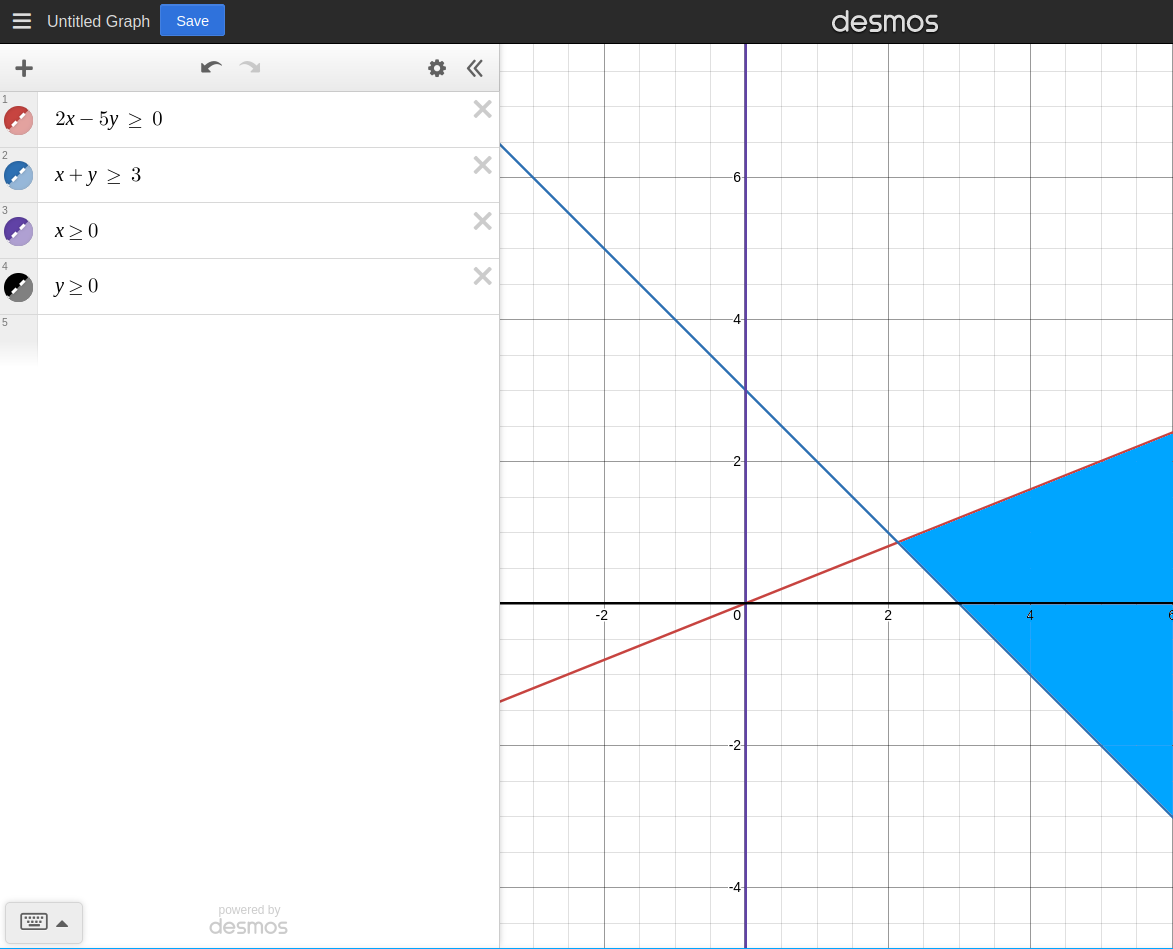
\includegraphics[scale=0.35]{desmos_lp_edited.png}
    \caption{A Desmos graphic of the lines representing the constraints of the above linear program (blue region).}
    \label{fig:desmos-lp}
\end{figure}
\paragraph{}Then we can draw lines parallel to the direction in which the objective function $f(x, y)$ increases which will be represented by vectors pointing in the direction: $$\nabla f(x,y) = (\frac{\partial f}{\partial x}, \frac{\partial f}{\partial y}) = (2,1)$$

\pagebreak

\begin{figure}
    \centering
    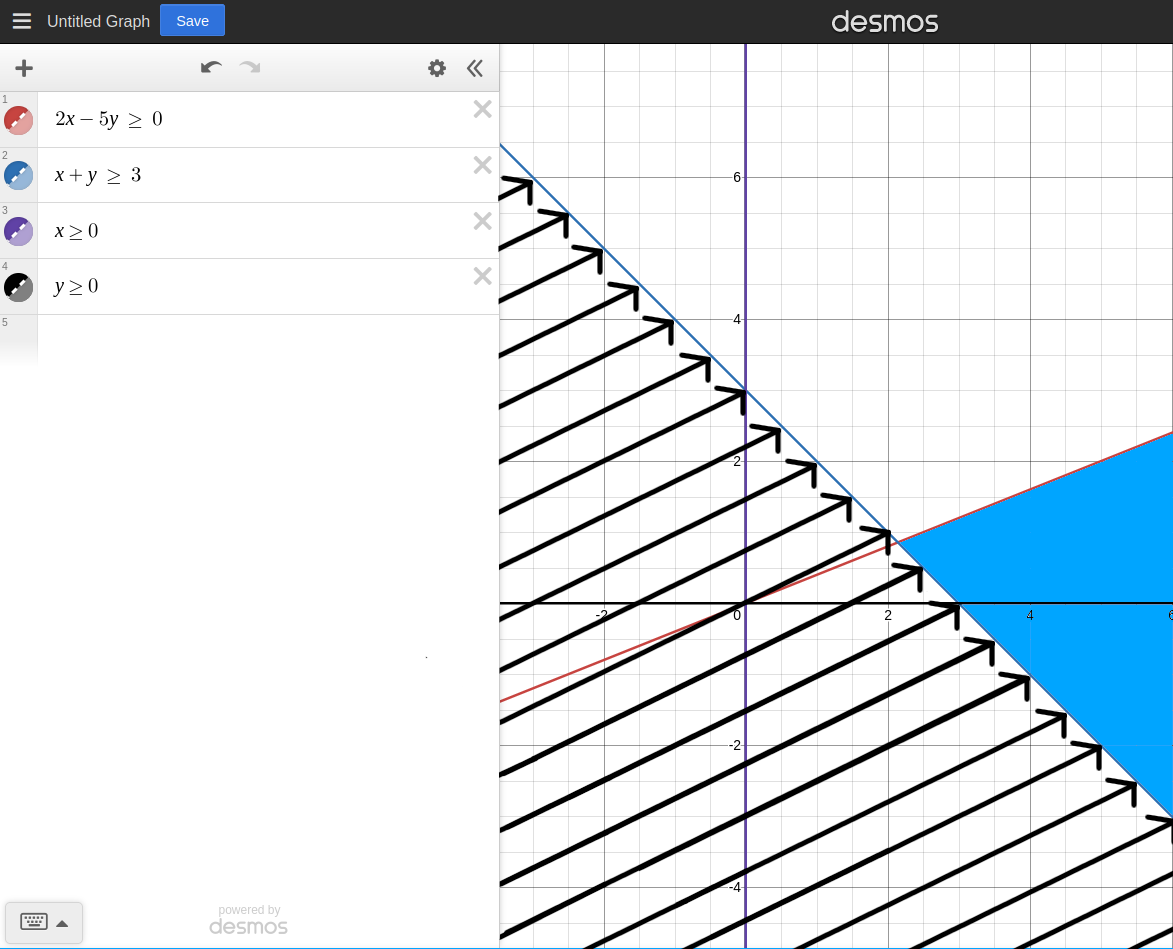
\includegraphics[scale=0.35]{desmos_lp_edited_2.png}
    \caption{A Desmos graphic of the lines representing the constraints of the above linear program (blue region) along with arrows denoting in which direction the objective function increases most.}
    \label{fig:enter-label}
\end{figure}

\paragraph{}Looking at these we want to minimise the total of the objective function given it is some point in the blue region, it is easy to notice that this exists on the lower-left edge of the region. Testing this we can look at the points of this edge which are described by the line:
\begin{equation*}
\begin{aligned}
y=-x + 3, & & \frac{15}{7} \leq x \leq 3
\end{aligned}
\end{equation*}

\paragraph{}Note that if we substitute this expression for the edge into $f(x, y)$ we get $$f(x,y(x)) = 2x + (-x + 3) = x + 3$$.
\paragraph{}So the objective function is non-constant along this line and is minimised by x being minimal. Hence the minimum value of the objective function along the given constraints is $x=\frac{15}{7}$ so $y=-(\frac{15}{7}) + 3 = \frac{6}{7}$.
\paragraph{}So finally we have found the solution to the linear program of $(x, y) = (\frac{15}{7}, \frac{6}{7})$ and this solution is unique.

\paragraph{}However, we cannot use the graphical method for problems with more than 3 variables as it is simply visually impossible to represent higher dimensional objects. However there is a method for solving such linear programs with similar intuitions called the simplex method.

\paragraph{}The core idea of the simplex method is that simple solutions to these linear programs can be found at the vertices of the shape described by the constraints of the program, moving between these vertices until an optimal solution can be found.

\paragraph{}This method will not be fully explained or derived here as it is a lengthy explanation.

\subsubsection{Setting up the damage optimisation program}
The following is the standard form of a linear program used for producing solutions:
\begin{equation*}
\begin{aligned}
    &\min & & \boldsymbol{cx} \\
    &\text{subject to} & & A\boldsymbol{x}=\boldsymbol{b}\\
    & & &\boldsymbol{x} \geq 0
\end{aligned}
\end{equation*}
Where A $\in \mathbb{R}^{m \times n}$, $\boldsymbol{x}$, $\boldsymbol{b}$, $\boldsymbol{c}$ $\in \mathbb{R}^n$, A represents the matrix of constraints while b and c represent the constraint equations and costs of each decision variable respectively. We however will constrain this problem to the integer space rather than the real space as it makes no sense to have "half a point" in a skill in the Dark Souls franchise.
\paragraph{}Hence the problem is now:
\begin{equation*}
\begin{aligned}
    &\min & & \boldsymbol{cx} \\
    &\text{subject to} & & A\boldsymbol{x}=\boldsymbol{b}\\
    & & &\boldsymbol{x} \geq 0
\end{aligned}
\end{equation*}
Where A $\in \mathbb{Z}^{m \times n}, \boldsymbol{x}, \boldsymbol{b}, \boldsymbol{c} \in \mathbb{Z}^n$.
\paragraph{}In order to create our linear program we need to identify what function we will be optimising and what constraints it is subject to. Obviously, we want to optimise the total damage output of a given weapon and we want to do this subject to the constraints of the levelling system in Dark Souls.
\subsubsection{Setting up the damage optimisation program - constraints}
\paragraph{}Firstly we will look at creating constraints for our linear program (as discussing the objective function will take much more time):
\begin{enumerate}
    \item We cannot have a skill be a higher level than 99,
    \item We cannot have a skill be below the maximum between what the class of the player starts at or what the minimum weapon requirement is for our given weapon.
    \item We must use all skill levels given to us, so the sum of all skill points must be equal to the default skill points in the skills and the number of skill points we will use.
\end{enumerate}
\par We can easily characterize these constraints using algebraic inequalities. Firstly let's define some notation that will help us (some of these will be reiterated in the next section):
\begin{itemize}
    \item Let $l$ be the number of skill points devoted to the problem.
    \item Let $c_i$ be the class minimum skill points for skill $i$.
    \item Let $r_i$ be the requirement for the given weapon to be used for skill $i$.
    \item Let $S$ be the set of all skills in the problem.
    \item Let $\boldsymbol{x}$ be the vector of skill points (each entry is related to some $i \in S$).
\end{itemize}
\par Now we can clearly write each of the three constraints algebraically as the following:
\begin{enumerate}
    \item $\boldsymbol{x} \leq 99$
    \item $x_i \geq \max\{c_i, r_i\}, \forall i \in S$
    \item $\sum_{i \in S}x_i =  l+ \sum_{i \in S} c_i$
\end{enumerate}
\subsubsection{Setting up the damage optimisation program - objective function}
\paragraph{}By looking at data mining efforts by the player-base of Dark Souls we have the exact formula used in calculating the damage of a given weapon in Dark Souls \cite{dswiki-formula}.
\paragraph{}Let's define some variables/constants to make this easier:
\begin{itemize}
\item Let $P = \{\text{STR},\text{DEX}\}$ be the set of physical attributes
\begin{itemize}
\item Write STR as 1, DEX as 2 throughout the project.
\end{itemize}
\item Let $M = \{\text{INT},\text{FTH}\}$ be the set of magic attributes
\begin{itemize}
\item Write INT as 3, FTH as 4 throughout the project.
\end{itemize}
\item Let $S = P \cup M$ be the set of damage attributes
\item Let $f_P$ be the damage rating function for physical attributes
\item Let $f_M$ be the damage rating function for magic attributes
\item Let $k_i \in (0,1]$ be the damage scaling multiplier of the skill $i \in S$ due to the given weapon
\item Let $B_P$ be the base physical damage of the given weapon
\item Let $B_M$ be the base magic damage of the given weapon
\end{itemize}

\paragraph{}Now by the efforts of the community \cite{dswiki-formula} the formula for the damage is:
\begin{equation}
f(\boldsymbol{x}) = B_P\cdot (1 + \sum_{i \in P} k_i f_P(x_i)) + B_M \cdot (1 + \sum_{i \in M} k_i f_M(x_i)
\end{equation}

\paragraph{}Where $\boldsymbol{x}$ is the vector of skill points of every skill $i \in S$. We want to simplify this down into the form $f(\boldsymbol{x})=\boldsymbol{c} \cdot \boldsymbol{x}$ where $\boldsymbol{c}$ is a vector of real numbers in order for this to be compatible with the simplex method for solving linear programs.

\paragraph{}Firstly we need to prove some properties of the simplex method that will help us prove that a simpler function will provide an equivalent solution to the linear program, firstly let's define a term.

\begin{definition}[Solution equivalency on a linear program] Let $f$, $g : \mathbb{R}^n \rightarrow \mathbb{R}$, $f$ and $g$ are called solution equivalent on a linear program $P$ if and only if solving $P$ with either $f$ or $g$ as the objective function provides the exact same solution to problem $P$ (where the constraints of $P$ are kept the same on both functions).
Let $\cong$ denote the solution equivalency between two functions on a linear program $P$.
\end{definition}


\begin{lemma}[Irrelevancy of linearity]
\label{ref:lemma_linearity}
Given a linear multi-variable function $f:\mathbb{R}^n\rightarrow\mathbb{R}$, two distinct functions $g_1$, $g_2 : \mathbb{R}^n\rightarrow\mathbb{R}$ of the form $g_1(\boldsymbol{x}) = a\cdot f(\boldsymbol{x}) + b$ $a$, $b \in \mathbb{R}$ and $a > 0$ are solution equivalent on any linear program.
\end{lemma}

\begin{proof}Let $f:\mathbb{R}^n\rightarrow\mathbb{R}$ and $g_1$, $g_2 : \mathbb{R}^n\rightarrow\mathbb{R}$ such that $g_1(\boldsymbol{x}) = a\cdot f(\boldsymbol{x}) + b$ where $a$, $b \in \mathbb{R}$ and $a > 0$ and $g_2(\boldsymbol{x}) = c\cdot f(\boldsymbol{x}) + d$ where $c$, $d \in \mathbb{R}$ and $c > 0$.

\paragraph{}Recall that solving linear programs involves following the optimising direction of the objective function until we meet a point in the feasible region which minimises the objective function. We find the optimising direction by taking the gradient of the objective function.

\paragraph{}Observe:
$$\nabla g_1 (\boldsymbol{x}) = \nabla (a \cdot f(\boldsymbol{x}) + b) = a\nabla f(\boldsymbol{x}) \text{ (By properties of partial derivatives)}$$
$$\nabla g_2 (\boldsymbol{x})= \nabla (c \cdot f(\boldsymbol{x}) + d) = c\nabla f(\boldsymbol{x}) \text{ (By properties of partial derivatives)}$$

\paragraph{}Now we may take the norm's of these vectors to get the unique direction's in which they point:
$$\nabla \hat g_1 (\boldsymbol{x}) = \frac{1}{|\nabla g_1(\boldsymbol{x})|} \nabla g_1(\boldsymbol{x})$$
$$\nabla \hat g_2 (\boldsymbol{x}) = \frac{1}{|\nabla g_2(\boldsymbol{x})|} \nabla g_2(\boldsymbol{x})$$
Now substituting each expression for gradient:
$$\nabla \hat g_1 (\boldsymbol{x}) = \frac{1}{|a \nabla f(\boldsymbol{x})|} a \nabla f(\boldsymbol{x}) = \frac{a}{a| \nabla f(\boldsymbol{x})|}  \nabla f(\boldsymbol{x}) = \frac{\nabla f(\boldsymbol{x})}{| \nabla f(\boldsymbol{x})|}$$
$$\nabla \hat g_2 (\boldsymbol{x}) = \frac{1}{|c \nabla f(\boldsymbol{x})|} c \nabla f(\boldsymbol{x}) = \frac{c}{c| \nabla f(\boldsymbol{x})|}  \nabla f(\boldsymbol{x}) = \frac{\nabla f(\boldsymbol{x})}{| \nabla f(\boldsymbol{x})|}$$

\paragraph{}Hence we get that each of the function $g_1$, $g_2$ point in the same direction, hence resulting in the same optimal solution given the same constraints of a linear program. So $g_1 \cong g_2$ on any linear program.
\end{proof}

\paragraph{}Using Lemma \ref{ref:lemma_linearity} we can rewrite the original function to be of the form $f(\boldsymbol{x})=\boldsymbol{c}\cdot \boldsymbol{x}$.
\paragraph{}Observe:
$$f(\boldsymbol{x}) = B_P\cdot (1 + \sum_{i \in P} k_i f_P(x_i)) + B_M \cdot (1 + \sum_{i \in M} k_i f_M(x_i)$$
$$\iff f(\boldsymbol{x}) = B_P + B_P \sum_{i \in P} k_i f_P(x_i) + B_M + B_M \sum_{i \in M} k_i f_M(x_i)$$
$$\iff f(\boldsymbol{x}) \cong B_P\sum_{i \in P} k_i f_P(x_i) + B_M\sum_{i \in M} k_i f_M(x_i)$$
$$\iff f(\boldsymbol{x}) \cong (k_1 B_P, k_2 B_P, k_3 B_M, k_4 B_M)\cdot (f_P (x_1), f_P(x_2), f_M(x_3), f_M(x_4))$$

\paragraph{}Hence we can instead solve the linear program using: 
\begin{equation}\textbf{}
    g(\boldsymbol{x})=(k_1 B_P, k_2 B_P, k_3 B_M, k_4 B_M)\cdot (f_P (x_1), f_P(x_2), f_M(x_3), f_M(x_4))
\end{equation}
\paragraph{}Notice that we are still not at the correct form. Here we run into some issues trying to further simplify the function. If $f_P$ and $f_M$ were perfectly linear functions then we could do that easily, however the definitions of the two functions are as follows \cite{dswiki-formula}:
\begin{equation}
f_{P}(x)=
    \begin{cases}
        0.005x & \text{if } 1 \leq x \leq 10 \\
        0.05 + 0.035(x-10) & \text{if } 10 < x \leq 20 \\
        0.4 + 0.0225(x-20) & \text{if } 20 < x \leq 40 \\
        0.85 + 0.0025(x-40) & \text{if } 40 < x < 99 \\
        1 & \text{if } x = 99 \\
        0 & \text{otherwise}
    \end{cases}
\end{equation}
\begin{equation}
f_{M}(x)=
    \begin{cases}
        0.005x & \text{if } 1 \leq x \leq 10 \\
        0.05 + 0.0225(x-10) & \text{if } 10 < x \leq 30 \\
        0.5 + 0.015(x-30) & \text{if } 30 < x \leq 50 \\
        0.8 + 0.0041(x-50) & \text{if } 50 < x < 99 \\
        1 & \text{if } x = 99 \\
        0 & \text{otherwise}
    \end{cases}
\end{equation}
\paragraph{}So the functions are actually continuous\footnote{$f_M$ is technically not continuous as it is laid out here as the 0.0041 coefficient on the interval $50 < x < 99$ is an approximation of the true coefficient for nice layout, the function itself is actually continuous.} and linear (assuming x is real and not discrete like it will be), but only over parts of their domain due to their piece-wise definitions. The reason for this is a concept known as "soft caps" in skill leveling in Dark Souls (This allows for very accurate damage optimisation). Hence we need to discuss some alternative ways to approach this linear program.
\section{Problems in linear programming}
\par In order to solve our optimisation for damage we must be able to properly handle the fact that the objective function changes as our decision variables change. These are different for each of the two subsets of skills $P$ and $M$.
\par One way we may handle this is by approximation of each function to a constant function allowing us to apply the simplex method without any problems, however we lose the previously mentioned encoded "soft caps" in skill leveling with this, although this will result in faster time to solve.
\par Another way we may handle this is by running the simplex method recursively on the problem every time the objective function changes due to the interval $x_i$ exists in for one of the skills $i \in S$, then by appropriately modifying the simplex method instance and continuing to solve until this happens again or the problem is solved. However this would cause an upper bound of 16 simplex method switches occurring, this also may not be guaranteed to provide a solution every-time (as I haven't proven this to be true).
\subsection{Solving the problem}
\par Let's try to solve this problem with the outlined solutions above.
\subsubsection{Approximation to a constant}
\par To approximate $f_P$ and $f_M$ to a constant function the easiest and most obvious solution will be to find the average (mean) value of the function and choosing that to be the approximation. This can be done by using the Mean Value of a Function formula \cite{mean-value-func}:
\begin{equation}
    \overline{f(x)}=\frac{1}{b-a}\int_{a}^{b}f(x)dx
\end{equation}
\par Hence we can compute the mean values of $f_P$ and $f_M$:
(I will show the steps for the first computation so there's an idea of where I got the constants)
\par Observe:
$$\overline{f_P(x)}=\frac{1}{99-1}\int_{1}^{99}f_P(x)dx$$
$$=\frac{1}{98}[\int_{1}^{10}f_P(x)dx + \int_{10}^{20}f_P(x)dx + \int_{20}^{40}f_P(x)dx + \int_{40}^{99}f_P(x)dx]$$
$$=\frac{1}{98}[\int_{1}^{10}0.005xdx + \int_{10}^{20}0.05 + 0.035(x-10)dx + \int_{20}^{40}0.4 + 0.0225(x-20)dx + \int_{40}^{99}0.85+0.0025(x-40)dx]$$
$$=\frac{1}{98}[(\frac{0.005}{2}x^2)\Big|_1^{10} + ( \frac{0.035}{2}x^2-9.95x)\Big|_{10}^{20} + (\frac{0.0225}{2}x^2-19.6x)\Big|_{20}^{40} + (\frac{0.0025}{2}x^2-39.15x)\Big|_{40}^{99}]$$
$$=\frac{1}{98}[0.2475 + 2.25 + 2.875 + 54.5013]$$
$$ = \frac{59.8738}{98}$$
$$ \approx 0.612 \text{to 3 s.f}$$
\par Now for the other function:
$$\overline{f_M(x)}=\frac{1}{99-1}\int_{1}^{99}f_M(x)dx$$
$$  \approx 0.642 \text{to 3 s.f}$$

\par We get that the averages of the two functions are similar so the approximation may not be great, but that is to be decided by test suites of optimisation problems later on.

\par From here we can apply the simplex method without problem so this is our first working solution for the problem.

\subsubsection{Recursive application of the simplex method on a piece-wise linear function}
\par Firstly it's easy to see that this will take a bit more work, however it will be a more useful algorithm due to the "soft caps" of Dark Souls being directly built into this rather than being ignored in the previous solution (although this may not affect the solution provided by the method).

\par In order to provide this 

\printbibliography[heading=bibintoc, title={Bibliography}]
\end{document}
